\documentclass[11pt]{jarticle}
\usepackage{ITCannual}
\usepackage{amsmath}
\usepackage{amssymb}
\usepackage{times}
\usepackage{graphicx}

%\usepackage[style=numeric]{biblatex}

\title{データ科学研究部門 研究報告}
\author{小林博樹, 鈴村豊太郎, 松島慎, 空閑洋平, 姜仁河, 川瀬純也, 華井雅俊, XXX, 他X名}

\begin{document}
\maketitle

\section{データ科学研究部門 概要}
データ科学研究部門では、2021年度、教授4名(特任教授1名)、准教授3名(特任准教授1名)、講師3名(特任講師3名)、助教 4 名(特任助教2名)が在籍した。同部門のメンバーは専任教員と特任教員の2つのグループから成る。専任教員はそれぞれが独立して研究活動を行うグループで、特任教員は石川特任教授を中心とする石川研究室グループである。 

%データ科学研究部門では、2019年度、助教 1 名。2020年度、教授2名(特任教授1名)、准教授2名(特任准教授1名)、講師3名(特任講師3名)、助教 6 名(助教1名は途中から兼任として在籍。助教1名は11月着任。特任助教3名)が在籍した。同部門のメンバーは専任教員と特任教員の2つのグループから成る。専任教員はそれぞれが独立して研究活動を行うグループで、特任教員は石川特任教授を中心とする石川研究室グループである。 


\subsection{専任教員グループの研究テーマ}

%計算機を介した人と生態系のインタラクションの研究(小林)\\
%解釈可能な機械学習手法の効率的な計算手法についての研究(松島)\\
%データ駆動型人文学研究の実践(中村)\\
%データ駆動型知能に基づくアーバンコンピューティング(姜)\\
%野生動物ワイヤレスセンサネットワーク実証実験基盤構築に向けた研究(川瀬)\\


\subsection{石川研究室全体の研究活動概要}

\section{データ科学研究部門 成果要覧}
\begin{招待講演}{1}

\bibitem{04末石智大01}
末石智大:高速光学系制御に基づくダイナミックビジョンシステムとその応用,第3回産業ロボット関連技術の標準化学術研究会,2022.

\bibitem{ykuga36619767}
空閑洋平, mdx: データ活用社会創成プラットフォーム構築の現状と今後, CloudWeek 2021@Hokkaido University, 2 Sep, 2021.

\bibitem{ykuga36619729}
空閑洋平, NetTLP: ハードウェアと協調動作可能なソフトウェアPCIeデバイス開発環境, 情報処理学会 FIT 情報科学技術フォーラム トップコンファレンスセッション, 26 Aug, 2021.



%\bibitem{suzumura-mdx2022}
%Toyotaro Suzumura, Akiyoshi Sugiki, Hiroyuki Takizawa, Akira Imakura, Hiroshi Nakamura, Kenjiro Taura, Tomohiro Kudoh, Toshihiro Hanawa, Yuji Sekiya, Hiroki Kobayashi, Shin Matsushima, Yohei Kuga, Ryo Nakamura, Renhe Jiang, Junya Kawase, Masatoshi Hanai, Hiroshi Miyazaki, Tsutomu Ishizaki, Daisuke Shimotoku, Daisuke Miyamoto, Kento Aida, Atsuko Takefusa, Takashi Kurimoto, Koji Sasayama, Naoya Kitagawa, Ikki Fujiwara, Yusuke Tanimura, Takayuki Aoki, Toshio Endo, Satoshi Ohshima, Keiichiro Fukazawa, Susumu Date, Toshihiro Uchibayashi, "mdx: A Cloud Platform for Supporting Data Science and Cross-Disciplinary Research Collaborations", https://arxiv.org/abs/2203.14188

\bibitem{suzumura-nci2021}
鈴村豊太郎, “mdx: A platform for the data-driven future”、オーストラリア国立研究所NCI(National Computational Infrastructure)-Fujitsu HPC, Cloud and Data Futures Workshop, 2022年02月

\bibitem{suzumura-nanotec2021}
鈴村豊太郎, "データ活用社会創成プラットフォームmdxにおけるマテリアルズ・インフォマティクス研究・共創に向けて", 第20回ナノテクノロジー総合シンポジウム, 2022年01月

\bibitem{suzumura-canon2021}
鈴村豊太郎, "人工知能を支えるグラフニューラルネットワークの最新動向", 2021年度キャノングローバル戦略研究所主催「経済・社会との分野横断的研究会」, 2021年12月


\end{招待講演}

\begin{招待論文}{1}

\bibitem{02早川智彦01}
早川智彦,石川正俊,亀岡弘之:時速100km走行でのトンネル覆工コンクリート高解像度変状検出手法,建設機械施工,vol.73,no.8,pp.19-23,2021.

\bibitem{02早川智彦02}
早川智彦,望戸雄史,石川正俊,大西偉允,亀岡弘之:【大臣賞】時速100km走行での覆工コンクリート高解像度変状検出手法,土木施工,vol.62,no.7,p.146,2021.

\bibitem{04末石智大02}
Yuri Mikawa,Tomohiro Sueishi,Yoshihiro Watanabe,and Masatoshi Ishikawa:Dynamic Projection Mapping for Robust Sphere Posture Tracking Using Uniform / Biased Circumferential Markers,2022 IEEE Conference on Virtual Reality and 3D User Interfaces (VR2022),(TVCG Invited)2022.


\end{招待論文}

\begin{受賞}{1}

\bibitem{03黄守仁01}
村上健一,黄守仁,石川正俊,山川雄司:高速ビジュアルフィードバックを用いた高速3次元位置補償システムの開発,第22回計測自動制御学会システムインテグレーション部門講演会(SI2021),講演会論文集,pp.1403-1405,優秀講演賞,2021.

\bibitem{04末石智大03}
末石智大,石川正俊:手指高速トラッキングに向けた楕円群指輪マーカーの開発,第22回計測自動制御学会システムインテグレーション部門講演会(SI2021),講演会論文集,pp.1382-1387,優秀講演賞,2021.

\bibitem{kobayashi1-1}
小林博樹:情報通信技術の導入が困難なインフラ圏外空間を対象とした情報デザインとIoTの研究,ドコモ・モバイル・サイエンス賞 社会科学部門 優秀賞,2021/9.

\bibitem{kobayashi1-2}
Hill Hiroki Kobayashi, Radioactive Live Soundscape, Winner, Universal Design Expert, Institute for Universal Design KG, Germany, 2021/05.
\bibitem{JIANG3-1}
Renhe Jiang et al., "DL-Traff: Survey and Benchmark of Deep Learning Models for Urban Traffic Prediction", 30th ACM International Conference on Information and Knowledge Management (CIKM), Best Resource Paper Runner Up, 2021.

\end{受賞}

\begin{著書}{1}

\bibitem{05宮下令央01}
宮下令央:有名論文ナナメ読み「Shader Lamps: Animating Real Objects With Image-Based Illumination」,情報処理学会,情報処理,Vol.62,No.5 ,2021.


\end{著書}

\begin{雑誌論文}{1}

\bibitem{01石川正俊01}
川原大宙,妹尾拓,石井抱,平野正浩,岸則政,石川正俊:輪郭情報に基づくテンプレートマッチングを用いた重畳車両の高速トラッキング,計測自動制御学会論文集,58巻,1号,pp.21-30,2022.

\bibitem{01石川正俊02}
小山佳祐,堀邊隆介,安田博,万偉偉,原田研介,石川正俊:ワンボード・USB給電タイプの高速・高精度近接覚センサの開発とプリグラスプ制御の解析,日本ロボット学会誌,Vol.39,No.9,pp.862-865,2021.

\bibitem{01石川正俊03}
Masahiro Hirano,YujiYamakawa,Taku Senoo and Masatoshi Ishikawa:An acceleration method for correlation-based high-speed object tracking,Measurement Sensors,Vol.18,Article No.100258,2021.

\bibitem{01石川正俊04}
Masahiko Yasui,Yoshihiro Watanabe,and Masatoshi Ishikawa:Wide viewing angle with a downsized system in projection-type integral photography by using curved mirrors,Optics Express,Vol.29,Issue8,pp.12066-12080,2021.

\bibitem{01石川正俊05}
Ruimin Cao,Jian Fu,Hui Yang,Lihui Wang,and Masatoshi Ishikawa:Robust optical axis control of monocular active gazing based on pan-tilt mirrors for high dynamic targets,Optics Express,Vol.29,No.24,pp.40214-40230,2021.

\bibitem{02早川智彦03}
Kenichi Murakami,Tomohiko Hayakawa,and Masatoshi Ishikawa: Hybrid surface measuring system for motion-blur compensation and focus adjustment using a deformable mirror,Applied Optics,vol.61,Issue2,pp.429-438,2022.

\bibitem{02早川智彦04}
Yuki Kubota,Yushan Ke,Tomohiko Hayakawa,Yushi Moko,and Masatoshi Ishikawa:Optimal Material Search for Infrared Markers under Non-Heating and Heating Conditions,Sensors,Vol.21,Issue 19,Article No.6527,pp.1-17,2021.


\bibitem{04末石智大04}
Yuri Mikawa,Tomohiro Sueishi,Yoshihiro Watanabe,and Masatoshi Ishikawa:Dynamic Projection Mapping for Robust Sphere Posture Tracking Using Uniform/Biased Circumferential Markers,IEEE Transaction on Visualization and Computer Graphics,1-1,2021 (Early Access).

\bibitem{04末石智大05}
松本明弓,新田暢,末石智大,石川正俊:高速注視点推定を用いた広域高解像度投影システムの実現,計測自動制御学会論文集,Vol.58,No.1,pp.42-51,2022.

\bibitem{05宮下令央02}
井倉 幹大,宮下令央,山下 淳,石川 正俊,淺間 一:高速点滅LEDマーカと複数のRGB-Dセンサを用いた遮蔽領域を提示可能な任意視点重畳映像生成システム,精密工学会誌,Vol. 88,No.3,2022.

\bibitem{05宮下令央03}
Leo Miyashita,Akihiro Nakamura,Takuto Odagawa,and Masatoshi Ishikawa: BIFNOM Binary-Coded Features on Normal Maps,Sensors,Vol.21,No.10,Article No.3469,2021.


\bibitem{06田畑智志01}
Hongjin Xu,Lihui Wang,Satoshi Tabata,Yoshihiro Watanabe,and Masatoshi Ishikawa:Extended depth-of-field projection method using a high-speed projector with a synchronized oscillating variable-focus lens,Applied Optics,Vol.60,Issue 13,pp.3917-3924,2021.

\bibitem{08金賢梧01}
Hyuno Kim,and Masatoshi Ishikawa:Sub-Frame Evaluation of Frame Synchronization for Camera Network Using Linearly Oscillating Light Spot,Sensors,Vol.21,Issue 18,Article No.6148,pp.1-14,2021.

\bibitem{ykuga36595746}
Yukito Ueno, Ryo Nakamura, Yohei Kuga, Hiroshi Esaki, A NIC-driven Architecture for High-speed IP Packet Forwarding on General-purpose Servers, Journal of Information Processing, 30, pp226-237, 2022.

\bibitem{JIANG1-1}
Renhe Jiang, Zekun Cai, Zhaonan Wang, Chuang Yang, Zipei Fan, Quanjun Chen, Xuan Song, and Ryosuke Shibasaki, "Predicting Citywide Crowd Dynamics at Big Events: A Deep Learning System", ACM Trans. Intell. Syst. Technol. (TIST), 13, 2, Article 21, April 2022.
\bibitem{JIANG1-2}
Zipei Fan, Chuang Yang, Zhiwen Zhang, Xuan Song, Yinghao Liu, Renhe Jiang, Quanjun Chen, and Ryosuke Shibasaki, "Human Mobility-based Individual-level Epidemic Simulation Platform", ACM Trans. Spatial Algorithms Syst. (TSAS), 8, 3, Article 19, September 2022.
\bibitem{JIANG1-3}
Chuang Yang, Zhiwen Zhang, Zipei Fan, Renhe Jiang, Quanjun Chen, Xuan Song, Ryosuke Shibasaki, "EpiMob: Interactive Visual Analytics of Citywide Human Mobility Restrictions for Epidemic Control", IEEE Transactions on Visualization and Computer Graphics (TVCG), 2022.
\bibitem{JIANG1-4}
Renhe Jiang, Zekun Cai, Zhaonan Wang, Chuang Yang, Zipei Fan, Quanjun Chen, Kota Tsubouchi, Xuan Song, Ryosuke Shibasaki, "DeepCrowd: A Deep Model for Large-Scale Citywide Crowd Density and Flow Prediction", IEEE Transactions on Knowledge and Data Engineering (TKDE), 2021.
\bibitem{JIANG1-5}
Jinliang Deng, Xiusi Chen, Zipei Fan, Renhe Jiang, Xuan Song, and Ivor W. Tsang, "The Pulse of Urban Transport: Exploring the Co-evolving Pattern for Spatio-temporal Forecasting", ACM Trans. Knowl. Discov. Data (TKDD), 15, 6, Article 103, May 2021.
\bibitem{HNakamura1}
山下智也,宮本大輔,関谷勇司,中村宏, ``通信挙動に基づいたスキャン攻撃検
知'', 情報処理学会論文誌~デジタル社会の情報セキュリティとトラスト~特集
号,11pages, Vol.62,No.12,pp.67-83


\end{雑誌論文}

\begin{査読付}{1}


\bibitem{01石川正俊06}
Hiromichi Kawahara,Taku Senoo,Idaku Ishii,Masahiro Hirano,Norimasa Kishi and Masatoshi Ishikawa:High-speed tracking for overlapped vehicles using Instance Segmentation and contour deformation,2022 IEEE/SICE International Symposium on System Integration (SII2022),Proceedings,pp.730-735,2022.

\bibitem{01石川正俊07}
石川正俊:高速ビジョンを用いた高速知能ロボット,ロボット,No.263,pp.56-58 ,2021.

\bibitem{01石川正俊08}
石川正俊:情報科学技術の構造と情報教育,IDE 現代の高等教育,2021年8-9月号,No.633,pp.9-13,2021.

\bibitem{01石川正俊09}
Masahiro Hirano,Yuji Yamakawa,Taku Senoo,Norimasa Kishi,Masatoshi Ishikawa:Multiple Scale Aggregation with Patch Multiplexing for High-speed Inter-vehicle Distance Estimation,IEEE Intelligent Vehicles Symposium (IV),Proceedings,pp.1436-1443,2021.

\bibitem{01石川正俊10}
Hirofumi Sumi,Hironari Takehara,Jun Ohta,and Masatoshi Ishikawa:Advanced Multi-NIR Spectral Image Sensor with Optimized Vision Sensing System and Its Impact on Innovative Applications,2021 Symposium on VLSI Technology ,2021 Symposium on VLSI Technology Digest of Technical Papers,JFS4-8,pp.1-2,2021.

\bibitem{01石川正俊11}
Masahiko Yasui,Yoshihiro Watanabe,and Masatoshi Ishikawa:Dynamic and Occlusion-Robust Light Field Illumination,ACM SIGGRAPH ASIA 2021 Posters (SIGGRAPH ASIA 2021),Proceedings,Article No.35,pp.1–2,2021.

\bibitem{02早川智彦05}
Yuki Kubota,Tomohiko Hayakawa,Osamu Fukayama,and Masatoshi Ishikawa:Sequential estimation of psychophysical parameters based on the paired comparisons,2022 IEEE/SICE International Symposium on System Integration (SII 2022),pp.150-154,2022.

\bibitem{02早川智彦06}
Ke Yushan,Yushi Moko,Yuka Hiruma,Tomohiko Hayakawa,and Masatoshi Ishikawa:Silk printed retroreflective markers for infrastructure maintenance vehicles in tunnels,SPIE Smart Structures + NDE On Demand,2022 (accepted).

\bibitem{03黄守仁02}
Mamoru Oka,Kenichi Murakami,Shouren Huang,Hirofumi Sumi,Masatoshi Ishikawa and Yuji Yamakawa:High-speed Manipulation of Continuous Spreading and Aligning a Suspended Towel-like Object,2022 IEEE/SICE International Symposium on System Integration,2022.

\bibitem{04末石智大06}
Tomohiro Sueishi and Masatoshi Ishikawa:  Ellipses Ring Marker for High-speed Finger Tracking,The 27th ACM Symposium on Virtual Reality Software and Technology (VRST2021) (Osaka),Proceedings,Article No. 31,pp.1-5,2021.


\bibitem{04末石智大07}
Soichiro Matsumura,Tomohiro Sueishi,Shoji Yachida,and Masatoshi Ishikawa:Eye Vibration Detection Using High-speed Optical Tracking and Pupil Center Corneal Reflection,The 43rd Annual International Conference of the IEEE Engineering in Medicine and Biology Society (EMBC2021) (Virtual)/Proceedings,ThDT3.5,2021.

\bibitem{04末石智大08}
Ayumi Matsumoto,Tomohiro Sueishi,and Masatoshi Ishikawa:High-speed Gaze-oriented Projection by Cross-ratio-based Eye Tracking with Dual Infrared Imaging,2022 IEEE Conference on Virtual Reality and 3D User Interfaces Abstracts and Workshops (VRW2022),Proceedings,pp.594-595,2022.

\bibitem{04末石智大09}
Tomohiro Sueishi,Soichiro Matsumura,Shoji Yachida,and Masatoshi Ishikawa: Optical and Control Design of Bright-pupil Microsaccadic Artificial Eye,2022 IEEE/SICE International Symposium on System Integration (SII2022) Online,Proceedings,pp.760-765,2022.

\bibitem{05宮下令央04}
Leo Miyashita,Kentaro Fukamizu,and Masatoshi Ishikawa:Simultaneous Augmentation of Textures and Deformation Based on Dynamic Projection Mapping,SIGGRAPH Asia 2021,Real Time Live!,2021.

\bibitem{05宮下令央05}
Leo Miyashita,Kentaro Fukamizu,and Masatoshi Ishikawa: Simultaneous Augmentation of Textures and Deformation Based on Dynamic Projection Mapping,SIGGRAPH Asia 2021,Emerging Technologies,2021.

\bibitem{05宮下令央06}
Leo Miyashita,Yohta Kimura,Satoshi Tabata,and Masatoshi Ishikawa:High-speed simultaneous measurement of depth and normal for real-time 3D reconstruction,SPIE Optical Engineering + Applications,2021.

\bibitem{06田畑智志02}
Yuping Wang,Senwei Xie,Lihui Wang,Hongjin Xu,Satoshi Tabata,and Masatoshi Ishikawa:ARSlice: Head-Mounted Display Augmented with Dynamic Tracking and Projection,The 10th international conference on Computational Visual Media (CVM 2022),2022(accepted).

\bibitem{09李ソ賢01}
Seohyun Lee,Hyuno Kim,Hideo Higuchi,and Masatoshi Ishikawa:Classification of Metastatic Breast Cancer Cell Using Deep Learning Approach,2021 International conference on artificial intelligence in information and communication (ICAIIC),Proceedings,pp.425-428,2021.

\bibitem{kobayashi2-1}
Keijiro Nakagawa, Daisuk\'e Shimotoku, Junya Kawase and Hill Hiroki Kobayashi, "Sustainable Wildlife DTN: Wearable Animal Resource Optimization through Intergenerational Multi-hop Network Simulation.", Proceedings of 2021 17th International Conference on Wireless and Mobile Computing, Networking and Communications (IEEE WiMob), 2021.
\bibitem{kobayashi2-2}
Daisuk\'e Shimotoku, Junya Kawase, Herv\'e Glotin and Hill Hiroki Kobayashi, "Comparison Between Manual and Automated Annotations of Eco-Acoustic Recordings Collected in Fukushima Restricted Zone.", Proceedings of 2021 International Conference on Human-Computer Interaction (HCII 2021), 2021.  
\bibitem{ykuga33191433}
Yukito Ueno, Ryo Nakamura, Yohei Kuga, Hiroshi Esaki, P2PNIC: High-Speed Packet Forwarding by Direct Communication between NICs, IEEE INFOCOM 2021 - IEEE Conference on Computer Communications Workshops (INFOCOM WKSHPS), pp1-6, May, 2021.

\bibitem{ykuga32183289}
Hajime Tazaki, Akira Moroo, Yohei Kuga, Ryo Nakamura, How to design a library OS for practical containers?, Proceedings of the 17th ACM SIGPLAN/SIGOPS International Conference on Virtual Execution Environments, 16 Apr, 2021.

\bibitem{JIANG2-1}
Zhaonan Wang, Renhe Jiang, Hao Xue, Flora Salim, Xuan Song, Ryosuke Shibasaki, "Event-Aware Multimodal Mobility Nowcasting", Proceedings of Thirty-Sixth AAAI Conference on Artificial Intelligence (AAAI), 2022.
\bibitem{JIANG2-2}
Zhaonan Wang, Renhe Jiang, Zekun Cai, Zipei Fan, Xin Liu, Kyoung-Sook Kim, Xuan Song, Ryosuke Shibasaki, "Spatio-Temporal-Categorical Graph Neural Networks for Fine-Grained Multi-Incident Co-Prediction", Proceedings of 30th ACM International Conference on Information and Knowledge Management (CIKM), 2021.
\bibitem{JIANG2-3}
Renhe Jiang, Du Yin, Zhaonan Wang, Yizhuo Wang, Jinliang Deng, Hangchen Liu, Zekun Cai, Jinliang Deng, Xuan Song, Ryosuke Shibasaki, "DL-Traff: Survey and Benchmark of Deep Learning Models for Urban Traffic Prediction", Proceedings of 30th ACM International Conference on Information and Knowledge Management (CIKM), 2021.
\bibitem{JIANG2-4}
Renhe Jiang, Zhaonan Wang, Zekun Cai, Chuang Yang, Zipei Fan, Tianqi Xia, Go Matsubara, Hiroto Mizuseki, Xuan Song, Ryosuke Shibasaki, "Countrywide OD Matrix Prediction for COVID-19", Proceedings of the European Conference on Machine Learning and Principles and Practice of Knowledge Discovery in Databases (ECML PKDD), 2021. 
\bibitem{JIANG2-5}
Jinliang Deng, Xiusi Chen, Renhe Jiang, Xuan Song, Ivor W. Tsang, "ST-Norm Spatial and Temporal Normalization for Multi-variate Time Series Forecasting", Proceedings of 27th ACM SIGKDD Conference on Knowledge Discovery and Data Mining (KDD), 2021.
\bibitem{JIANG2-6}
Zhaonan Wang, Tianqi Xia, Renhe Jiang, Xin Liu, Kyoung-Sook Kim, Xuan Song, Ryosuke Shibasaki, "Forecasting Ambulance Demand with Profiled Human Mobility via Heterogeneous Multi-graph Convolution Network”, Proceedings of the 37th IEEE International Conference on Data Engineering (ICDE), 2021. 
\bibitem{HNakamura2}
Satoshi Okada, Daisuke Miyamoto, Yuji Sekiya, Hiroshi Nakamura, ``New
LDoS Attack in Zigbee Network and its Possible Countermeasures'', The
5th IEEE International Workshop on Big Data and IoT Security in Smart
Computing, 6pages, Aug.  2021

\bibitem{HNakamura3}
Shaswot Shresthamali, Masaaki Kondo, Hiroshi Nakamura, ``Multi-objective
Reinforcement Learning for Energy Harvesting Wireless Sensor Nodes'',
14th IEEE International Symposium on Embedded Multicore Many-core
Systems-on-Chip (MCSoC 2021), 8pages, Dec. 2021

\bibitem{HNakamura4}
Satoshi Okada, Daisuke Miyamoto, Yuji Sekiya, Hideki Takase, Hiroshi
Nakamura, ``LDoS Attacker Detection Algorithms in Zigbee Network'',
Proceedings of the 14th IEEE International Conference on Internet of
Things, Dec. 2021

\bibitem{HNakamura5}
Siyi Hu, Masaaki Kondo, Yuan He, Ryuichi Sakamoto, Hao Zhang, Jun Zhou
and Hiroshi Nakamura, ``GraphDEAR: An Accelerator Architecture for
Exploiting Cache Locality in Graph Analytics Applications'', Proc. of 30
Euromicro International Conference on Parallel, Distributed, and
Network-based Processing, Mar. 2022


\bibitem{suzumura-sc2021}
Venkatesan T. Chakaravarthy, Shivmaran S. Pandian, Saurabh Raje, Yogish Sabharwal, Toyotaro Suzumura, Shashanka Ubaru, 
"Efficient scaling of dynamic graph neural networks". SC2021(The International Conference for High Performance Computing, Networking, Storage, and Analysis)

\bibitem{suzumura-smds21}
Shilei Zhang, Toyotaro Suzumura, Li Zhang, "DynGraphTrans: Dynamic Graph Embedding via Modified Universal Transformer Networks for Financial Transaction Data", IEEE SMDS 2021 (International Conference on Smart Data Services) 
\end{査読付}

%\begin{公開}{1}
%
%
%\end{公開}
%
%\begin{特許}{1}
%
%
%\end{特許}

\begin{発表}{1}

\bibitem{01石川正俊12}
谷内田尚司,並木重哲,小川拓也,細井利憲,石川正俊:高速カメラ物体認識技術を用いた錠剤外観検査装置,製剤機械技術学会誌,Vol.30,No.4,pp.35-40,2021.

\bibitem{02早川智彦07}
栃岡 陽麻里,早川 智彦,石川 正俊:身体感覚と視覚情報にずれが生じる低遅延没入環境におけるターゲットの加速度がユーザへ与える影響,第26回日本バーチャルリアリティ学会大会 (VRSJ2021),論文集,3B2-3,2021.

\bibitem{03黄守仁03}
村上 健一,黄 守仁,石川 正俊,山川 雄司:高速ビジュアルフィードバックを用いた高速3次元位置補償システムの開発,第22回計測自動制御学会システムインテグレーション部門講演会 (SI2021),講演会論文集,pp.1403-1405,2021.

\bibitem{03黄守仁04}
岡衛,村上健一,黄守仁,角博文,石川正俊,山川雄司:面状柔軟物の展開に向けたコーナーの状態認識と把持動作計画,第39回日本ロボット学会学術講演会(RSJ2021),講演会論文集,3F1-01,2021.

\bibitem{03黄守仁05}
上野永遠,黄守仁,石川正俊:上腕の一自由度回転運動に向けた高周波電気刺激フィードバック制御システムの構築,第39回日本ロボット学会学術講演会(RSJ2021),講演会論文集,RSJ2021AC2J1-01,2021

\bibitem{03黄守仁06}
長谷川雄大,黄守仁,山川雄司,石川正俊:閉リンク機構を用いた動的補償モジュールの開発,第39回日本ロボット学会学術講演会(RSJ2021),講演会論文集,RSJ2021AC2D2-05,2021.

\bibitem{04末石智大10}
末石智大,石川正俊:手指高速トラッキングに向けた楕円群指輪マーカーの開発,第22回計測自動制御学会システムインテグレーション部門講演会(SI2021),講演会論文集,pp.1382-1387,2021.

\bibitem{04末石智大11}
末石智大,松村蒼一郎,谷内田尚司,石川正俊:マイクロサッカード高精度計測に向けた動的な明瞳孔眼球模型の開発,第22回計測自動制御学会システムインテグレーション部門講演会(SI2021),講演会論文集,pp.2011-2016,2021.

\bibitem{04末石智大12}
松村蒼一郎,末石智大,井上満晶,谷内田尚司,石川正俊:光学系制御撮影下の角膜反射法によるマイクロサッカード検出高精度化の検討,第22回計測自動制御学会システムインテグレーション部門講演会(SI2021),講演会論文集,pp.2025-2028,2021.

\bibitem{04末石智大13}
三河祐梨,末石智大,石川正俊:球体姿勢に対応した回転相殺テクスチャの高速投影の残像効果による一軸回転可視化法の提案,第26回日本バーチャルリアリティ学会大会(VRSJ2021),論文集,2D2-5,2021.

\bibitem{04末石智大14}
三河祐梨,末石智大,渡辺義浩,石川正俊:VarioLight2円周マーカを用いた球体への広域かつ遮蔽に頑健なダイナミックプロジェクションマッピング,第27回画像センシングシンポジウム(SSII2021),講演論文集 IS1-25,2021.

\bibitem{ykuga36616798}
塙敏博, 中村遼, 空閑洋平, 杉木章義, 田浦健次朗, データ利活用に向けた仮想化プラットフォームmdxの基本性能評価, 研究報告ハイパフォーマンスコンピューティング(HPC), 7, pp1-9, Mar, 2022.

\bibitem{ykuga36616852}
中村遼, 空閑洋平, AES67のソフトウェアによる実装の試行, 研究報告インターネットと運用技術(IOT), 54, pp1-4, Feb, 2022.

\bibitem{HNakamura6}
仮屋 郷佑, 坂本 龍一, 中村 宏, ``動的スケジューリングによるマイクロサー
ビスの実行最適化'', 情報処理学会コンピュータシステム・シンポジウム論文
集, 2021,pages. 1-10 (2021-11-25)


\bibitem{suzumura-axies2021}
鈴村豊太郎, "データ活用社会創成プラットフォームmdxの設計・実装・運用〜多様な学際領域における共創に向けて~", 大学ICT推進協議会2021年度年次大会(AXIES2021), 2021年12月
\end{発表}

%\begin{特記}{1}
%
%
%\end{特記}

\begin{報道}{1}

\bibitem{01石川正俊13}
石川正俊:「ロボット」100年で次へ 東大特任教授・石川正俊氏に聞く 人のはるかに先を行く 機械性能極限まで発揮,電波新聞,令和3年7月8日.

\bibitem{01石川正俊14}
石川正俊:「高速反応や自律航行 ロボット研究進む 東大でオンライン公開講座」,電波新聞,令和3年6月17日.

\bibitem{01石川正俊15}
石川グループ研究室:MBS毎日,日曜日の初耳学,「VarioLight2,ダイナミックプロジェクションマッピング」,令和3年9月13日.

\bibitem{01石川正俊16}
石川グループ研究室:テレビ東京,日経ニュースプラス9,「ElaMorph projection,VarioLight2,高速トンネル検査」,令和3年6月8日.

\bibitem{01石川正俊17}
石川グループ研究室:TBS,あさチャン!,「ジャンケンロボット,高速道路トンネル検査」,令和3年6月28日.


\end{報道}


\section{データ科学研究部門 教員研究活動}

\subsection{研究報告(小林 博樹)}
\input{Kobayashi/ITCannual-list-Kobayashi}

\subsection{研究報告(鈴村 豊太郎)}
\input{Suzumura/ITCannual-list-Suzumura}

\subsection{研究報告(松島 慎)}

本節では2021年度の松島研究室の研究活動について報告する。
弊研究室では知識発見のための機械学習手法の効率的な計算手法についての研究を推進してきた。
与えられたデータを用いて入力から出力を予測する方法論としての機械学習は特に深層学習モデルの学習手法の発展を通じて
高い精度での予測を実現できることが様々な分野で報告されている。
これらは画像の識別や多言語間の翻訳など、公開されたデータが豊富にあるタスクにおいて複雑な関数を学習する方法論である。
一方で、複雑な関数を機械が学習できることは必ずしも我々の画像や言語に対する理解を深めるわけではない。
現代社会には様々なデータが蓄積されており、データを上述の意味で利用するだけでなく、隠れた法則性や生成原理などの理解に結び付く属性間の関係を抽出することが求められる。
そのため、
我々はデータの関係を理解するのに有用なモデルとして以下の3つの分野に関する研究を行っている。
\begin{itemize}
    \item 一般化加法モデルに関する研究
    \item 組合せ線形モデルに関する研究
    \item 部分空間クラスタリングに関する研究
\end{itemize}
2021年度はさらに統計的因果探索と呼ばれる手法群について調査・研究を開始した。

統計的因果探索とは、変数間の単純な相関関係だけでなく因果関係にも着目し、属性間の構造を推定する手法である。
統計的因果探索において因果関係とは介入と呼ばれる変数の操作が他の変数の分布へどう影響を及ぼすかを表す概念である。例えば、特定の薬を服用したかどうかの変数に着目した時、
無作為に選んだ人に薬を服用させた場合、この変数への介入操作が行われたとみなすことができる。
その集団に関する他の変数の分布は介入後分布と呼ばれ条件付き分布は一般に別物である。

我々は統計的因果探索の手法の中でも、介入操作が行われたデータを使わずに、変数群の同時分布から無作為に抽出されたとみなされるデータから因果関係を推定する手法の調査・研究を行った。
前述した介入の定義によると介入操作の結果を得ない限りは因果関係の推定は不可能のように考えられるが、
データの生成過程が構造方程式モデルで記述できると仮定した場合は、同時分布からのデータのみから因果関係の推定が可能である場合がある。

一般に確率変数をノードとする有向グラフ$G=(V,E)$に関する構造方程式モデルとは、各$e_j$を互いに独立な確率変数とし、
各確率変数$X_{j}$を以下のような方程式系で表すものである:
\begin{align*}
    X_{j}=f_{j}\left(\mathbf{PA}(X_{j}), e_{j}\right), \quad j=1, \ldots, d
\end{align*}
ここで、$\mathbf{PA}(X_j)$は$G$で$X_j$の親となる確率変数の集合、$f_j$は考えている確率空間において可測な任意の関数である。

DAG (Directed Acyclic Graph)である$G=(V,E)$に関する構造方程式モデルが識別可能であるとは、同時分布からのデータのみから因果関係の推定、すなわちグラフ$G$の推定が可能であることを意味し、
特にLiNGAMモデルは識別可能な構造方程式モデルの部分集合としてよく知られているものである\cite{S}。本年度はLinGAMモデルの学習手法を検討し、実験的に既存手法を上回る精度を持つ手法の設計・開発を行った。今後この手法のさらなる精度改善や学習効率化を検討し、対外発表を行う予定である。

\begin{thebibliography}{9}
\bibitem{S} 
Shimizu, Shohei, et al. "A linear non-Gaussian acyclic model for causal discovery." Journal of Machine Learning Research 7.10 (2006).
%\bibitem{F} 
\end{thebibliography}

\input{Matsushima/ITCannual-list-Matsushima}

\subsection{研究報告(空閑 洋平)}
\input{Kuga/ITCannual-list-Kuga}

\subsection{研究報告(姜 仁河)}

モノのインターネット(IoT)、ビッグデータ、人工知能技術の急速な発展に伴い、スマートシティは新しい研究分野として政府や産業界から非常に重視されている。様々なマルチモーダルの人の流れ移動データと都市のビッグデータ(スマートフォン位置データ、携帯電話の通話記録データ、GPS 軌跡データ、都市交通網データ、自然災害データ、伝染病データ、公共健康データなど)を統合、処理、分析し、新世代の人工知能技術(深層学習、強化学習、アンサンブル学習など)と結び付け、都市規模の人の流れの移動についてのモデリング、シミュレーション、予測を実現することにより、都市の交通整理、都市における緊急事態管理、災害時の人道支援、伝染病の拡大予防対策、公共の健康促進などの実現を目指す。これを背景にし、2019年度および2020年度に、引き続き私はデータ駆動型知能とアーバンコンピューティングについて研究活動を行ってきた。お陰様で複数の研究成果\cite{JIANG1901,JIANG2001,JIANG2002,JIANG2003,JIANG1902,JIANG1903,JIANG1904,JIANG2004,JIANG2005,JIANG2006}をあげている。ここにて以下2点の研究プロジェクトをピックアップして詳しく紹介する。

\begin{itemize}
    \item 深層学習による都市全体の群衆密度・流れの予測
    \item モビリティデータと医療データを統合したインフルエンザ流行の解析・予測
\end{itemize}

\subsubsection{深層学習による都市全体の群衆密度・流れの予測}
大規模な都市区域を数々のきめ細かいメッシュグリッドへとメッシングすることで、連続的な期間における都市全体の群集や交通情報を映像のように表現し、各タイムスタンプを一枚の映像フレームとして扱うことができる(図\ref{fig:intro1_jiang})。この考え方に基づき、都市全体の群集や交通に関する映像型の予測に対応するため一連の手法が提案された。現在、この手法群の評価は (1) 一部のモデルは他のモデルと比較できない、(2) 一部のモデルは群集流動データではなくタクシーや自転車などの交通流量のみによって検証されている、(3) 一部のモデルは天候データやPOIデータなどの外部データ源を活用している、(4) 一部のモデルは独自に設計したオブジェクト関数を用いている、(5) ホットステーションや朝の混雑時間における住宅地域といった一部の具体的な地域や時間帯によるケーススタディが欠けている、といった観点から未だに不十分である。本研究を通じ、我々は実世界のスマートフォンによるアプリケーションを通じて生成した集合的な人の移動に関する新たなデータセットを公開し、複数のオープンデータセットに基づいてそのような種類のアーバンコンピューティング問題に対する標準的なベンチマークを構築することを試みる。具体的には、(1) 群集および交通の密度予測、流出入予測といった2種類の古典的な問題を対象として設定する。前者では次のタイムスタンプにおいて各メッシュグリッドに何人または何台いるかを予測し、後者では次の時間間隔において各メッシュグリッドに何人または何台が流入または流出するかを予測する。過去に観察した複数ステップ分のデータを入力として扱い、次のステップにおける予測結果を出力として報告する。(2) 広く普及しているスマートフォンのアプリによるGPSログデータを用いて実世界の群集密度や流動を反映する新規データセットを作成する。次に、作成した新規データセットと既存のデータセットを用いて群集および交通の予測を実施できる。(3) 統一した目的関数であるMSEをモデルの訓練に採用し、外部データ源や関連する処理モジュールをモデルから除外する。それにより、時空間データの映像型モデリングに関する純粋な能力を公平に検証することができる。(4) 選択した地域の時系列の予測結果をケーススタディとして追加し、異なる場所や時間に対する有効性を実証する。
\begin{figure}[h]
	\centering	
	\includegraphics[width=0.95\textwidth]{Kyo/figure/intro1.eps}
	\caption{都市全体の群集密度や流れは映像のように表現}
	\label{fig:intro1_jiang}
\end{figure}

\subsubsection{モビリティデータと医療データを統合したインフルエンザ流行の解析・予測}
インフルエンザの流行により、健康被害や社会経済への影響が大きいため、インフルエンザがいつどこで発生し、感染がどのように拡大するかは重要な課題として政府や自治体に強調された。ビッグデータ時代、特にIoT(Internet of Things)時代に、従来の医学・免疫学分野になかったデータ駆動の方法を利用し、インフルエンザ流行のメカニズムを解明する。さらにそのメカニズムに基づいて流行状況の高精度な予測モデルを構築する。具体的に、本研究はブログウォッチャーGPS軌跡データ(人の移動モビリティデータとNDBレセプトデータ(医療データ)を利用する。ブログウォッチャーGPS軌跡データとは、提携アプリをダウンロードし、位置情報の取得を許可したユーザーのスマートフォン端末から、GPSで補足した経度緯度の位置情報である。一方、NDBレセプトデータとは、情報データベース(NDB)に蓄積されたレセプト情報・薬の処方情報などであり、インフルエンザ感染数のproxyとなるデータでもある。この二つのデータを組み合わせて、過去十年間の感染の広がり方の差異と人的空間移動の状況を解析し、まず地域間の人の移動がインフルエンザ感染・流行に寄与しているかを検証する;そして、関連していることが確定されればその人の移動によるインフルエンザ流行のメカニズムに基づき、リアルタイムかつ高精度のインフルエンザ流行状況の予測モデルを構築する。なお、本研究について、1)データへのアクセス(個人情報などの課題);2)データの粒度の違い、仕様の違い;3)データ量の多さ;4)モデリング手法などのチャレンジを克服するために、GPS軌跡データとNDB医療データを同時に用意するだけでなく、それぞれのデータに高度な解析能力を持つ時空間データ専門家及び医療データ専門家の高度なコラボレーションも欠かせない。異分野のデータと異分野の専門知識を備えた上で、次世代の人工知能技術(深層学習、強化学習、アンサンブル学習など)に基づき、新型のデータ統合解析技術・AI予測モデルを開発する。本研究内容の概要は以下の図\ref{fig:intro2_jiang}にまとめている。

\begin{figure}[h]
	\centering	
	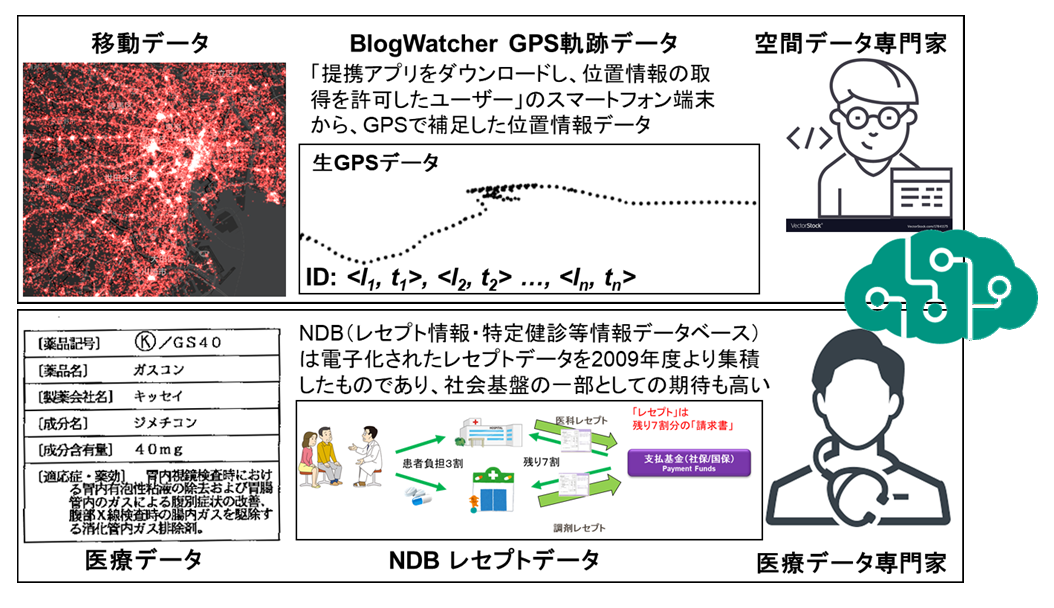
\includegraphics[width=0.95\textwidth]{Kyo/figure/intro2.eps}
	\caption{モビリティデータと医療データの統合解析}
	\label{fig:intro2_jiang}
\end{figure}
\begin{雑誌論文}{1}
\bibitem{JIANG1901}
Zipei Fan, Xuan Song, Renhe Jiang, Quanjun Chen, and Ryosuke Shibasaki:
Decentralized Attention-based Personalized Human Mobility Prediction, Proceedings of the ACM on Interactive Mobile Wearable and Ubiquitous Technologies, Vol.3, No.4, pp1-26, December 2019.
\bibitem{JIANG2001}
Zipei Fan, Xuan Song, Quanjun Chen, Renhe Jiang, Ryosuke Shibasaki, and Kota Tsubouchi:  
Trajectory fingerprint: one-shot human trajectory identification using Siamese network, CCF Transactions on Pervasive Computing and Interaction, 2(2), 113-125, 2020.
\bibitem{JIANG2002}
Renhe Jiang, Quanjun Chen, Zekun Cai, Zipei Fan, Xuan Song, Kota Tsubouchi, and Ryosuke Shibasaki: 
Will You Go Where You Search? A Deep Learning Framework for Estimating User Search-and-Go Behavior, Neurocomputing, 2020.
\bibitem{JIANG2003}
Renhe Jiang, Xuan Song, Zipei Fan, Tianqi Xia, Zhaonan Wang, Quanjun Chen, Zekun Cai, and Ryosuke Shibasaki: 
Transfer Urban Human Mobility via POI Embedding over Multiple Cities, ACM/IMS Trans. Data Sci. 2, 1, Article 4, 26 pages, January 2021.
\end{雑誌論文}

\begin{査読付}{1}
\bibitem{JIANG1902}
Renhe Jiang, Xuan Song, Dou Huang, Xiaoya Song, Tianqi Xia, Zekun Cai, Zhaonan Wang, Kyoung-Sook Kim, and Ryosuke Shibasaki:
Deepurbanevent: A system for predicting citywide crowd dynamics at big events, Proceedings of The 25th ACM SIGKDD International Conference on Knowledge Discovery \& Data Mining (KDD'19), pp2114-2122, July 2019.
\bibitem{JIANG1903}
Zipei Fan, Quanjun Chen, Renhe Jiang, Ryosuke Shibasaki, Xuan Song, and Kota Tsubouchi:
Deep Multiple Instance Learning for Human Trajectory Identification, Proceedings of the 27th ACM SIGSPATIAL International Conference on Advances in Geographic Information Systems (SIGSPATIAL'19), pp512-515, November 2019.
\bibitem{JIANG1904}
Xiaodan Shi, Xiaowei Shao, Zipei Fan, Renhe Jiang, Haoran Zhang, Zhiling Guo, Guangming Wu, Wei Yuan, and Ryosuke Shibasaki:
Multimodal Interaction-Aware Trajectory Prediction in Crowded Space, Proceedings of The Thirty-Fourth AAAI Conference on Artificial Intelligence (AAAI'20), pp11982-11989, February 2020.
\bibitem{JIANG2004}
Satoshi Miyazawa, Xuan Song, Renhe Jiang, Zipei Fan, Ryosuke Shibasaki, and Taisei Sato:
City-Scale Human Mobility Prediction Model by Integrating Gnss Trajectories and Sns Data Using Long Short-Term Memory, ISPRS Annals of the Photogrammetry, Remote Sensing and Spatial Information Sciences, Volume V-4-2020, 2020, pp.87-94, August 2020.
\bibitem{JIANG2005}
Quanjun Chen, Renhe Jiang, Chuang Yang, Zekun Cai, Zipei Fan, Kota Tsubouchi, Xuan Song, Ryosuke Shibasaki: 
DualSIN: Dual Sequential Interaction Network for Human Intentional Mobility Prediction, Proceedings of the 28th International Conference on Advances in Geographic Information Systems (SIGSPATIAL '20), pp.283–292, November 2020.
\bibitem{JIANG2006}
Xiaodan Shi, Xiaowei Shao, Guangming Wu, Haoran Zhang, Zhiling Guo, Renhe Jiang, Ryosuke Shibasaki: 
Social-DPF: Socially acceptable distribution prediction of futures, Proceedings of The Thirty-Fifth AAAI Conference on Artificial Intelligence (AAAI'21), February 2021.
\end{査読付}




\subsection{研究報告(川瀬 純也)}
\input{Kawase/ITCannual-list-Kawase}

\subsection{研究報告(華井 雅俊)}
\input{Hanai/ITCannual-list-Hanai}

% Ishikawa group

\end{document}

